
\documentclass[11pt,a4paper,slovene]{article}

%Uporabljeni paketi
\usepackage[slovene]{babel}
\usepackage[utf8]{inputenc}
\usepackage{lmodern}
\usepackage[T1]{fontenc}
\usepackage{fancyhdr}
\usepackage{caption}
\captionsetup{font={default,footnotesize}, labelfont=bf, format=hang,indention=.0cm}
\usepackage{graphicx,epsfig}
\usepackage{amsmath}
\usepackage{multirow}
\usepackage{color}
\usepackage{url}
\usepackage{makeidx}
\usepackage[official]{eurosym}

\usepackage{hyperref}
\hypersetup{
   bookmarksnumbered=true,
   urlbordercolor={0 1 0},
   linkbordercolor={1 1 1},
   unicode=true,
   pdftitle={ Brez\v{z}i\v{c}na in Mobilna Omre\v{z}ja },
   pdfauthor={Asistent},
   pdfdisplaydoctitle=true,
   pdftoolbar=true,
   pdfmenubar=true,
   pdfstartview=X Y Z
}

\urlstyle{same}

\setlength{\parskip}{12pt}
\setlength\parindent{0pt}
\setlength\unitlength{1mm}

\begin{document}
\label{naslov}
\pdfbookmark[1]{Naslov}{naslov}
\thispagestyle{empty}

\begin{center}
\begin{Large}
Brez\v{z}i\v{c}na in Mobilna Omre\v{z}ja\\
Študijsko leto 2015/2016\\
\end{Large}

\vspace*{4cm}
\begin{LARGE}
\textbf{Indoor lokalizacija\\}
\end{LARGE}
\vspace*{0.5cm}

\begin{Large}
Končno poročilo seminarske naloge\\

\vspace*{4cm}

Miha Novak\\
Vpisna št. 63099999\\
Klemen Škoda\\
Vpisna št. 63100318\\

\vspace*{5cm}
Ljubljana, \today
\end{Large}
\end{center}

\pagebreak
\setcounter{page}{1}
\pagenumbering{arabic}


\label{Kazalo}
\pdfbookmark[1]{Kazalo}{Kazalo}
\tableofcontents
\thispagestyle{empty}
\pagebreak

\section{Uvod in motivacija}
V današnjem času zelo veliko uporabljamo GPS kot pomoč pri iskanju poti do lokacij. Problem pa nastane, v zaprtih prostorih, kjer je GPS zelo nenatančen oz. neuporaben.
Z našo aplikacijo želimo pokazati primer iskanja lokacije v zaprtih prostorih. Taka rešitev bi bila zelo uporabna v velikih nakupovalnih središčih ter naprimer skladiščih, da se lažje orienteramo in najdemo željeno lokacijo. Največjo uporabnost pa vidimo v primerih klicov v sili, saj se velikokrat zgodi, da je zelo težko najti osebo v stanovanjskem objektu, saj je večinoma vedno podan le naslov ne pa točna lokacija. Zato mislimo, da bi z nadaljno implementacijo in razširitvijo naše aplikacije lahko naredili zelo uporabno in dobro rešitev, ki bi pomagala mnogim.
Opis problema, ki ga naša rešitev reši.

\section{Opis uporabljene strojne in programske opreme}

\subsection{Linksys WRT54GL \cite{wrt}}
Linksys je leta 2005 poslal na trg usmerjevalnik WRT54GL 1.1, ki podpira tudi third-party firmware-e. Usmerjevalnik WRT54GL 1.1 podpira 802.3 ethernet in 802.11b/g wireless. Sestavljajo ga 4 + 1 portna stikala, WAN port je privzeto na drugem VLAN-u kot ostali, 2 zunanji anteni (TNC konektor), CPU broadcom BCM4704 (264MHZ), 16MB RAM-a in 4MB flash pomnilnika.\newline
Privzeto je naložen VxWorks firmware, ki pa močno omejuje konfiguriranje usmerjevalnika in ne podpira CLI vmesnika, kar pomeni, da ga lahko konfiguriramo samo preko web vmesnika. WRT54GL podpira namestitev third-party linux firmware-a. Namestimo lahko OpenWRT, DD-WRT, HyperWRT, Tomato, Tarifa in še mnoge druge firmware-e. Pri naši analizi omrežja smo uporabljali privzeti in tudi OpenWRT firmware.


\subsection{Nexus 5 \cite{nexus}}
Nexus 5 je kombinacija strojne opreme za katero je poskrbel LG ter naprednih programskih rešitev in storitev Googla. Nexus 5, z štirijedernim procesorjem Snapdragon 800, ima naložen androido 6.0 (Marshmallow), povezati pa se zna v vsa mobilna omrežja (4G/LTE).

\subsection{Android Studio \cite{android}}
Android Studio je uradno razvojno orodje za razvijanje Android aplikacij. Android studio sestavljajo
\begin{enumerate}
\item Ukazna vrstica
\item Navigacijska vrstica
\item Urejevalnik
\item Orodja
\item Okno za obvestila
\end{enumerate} 

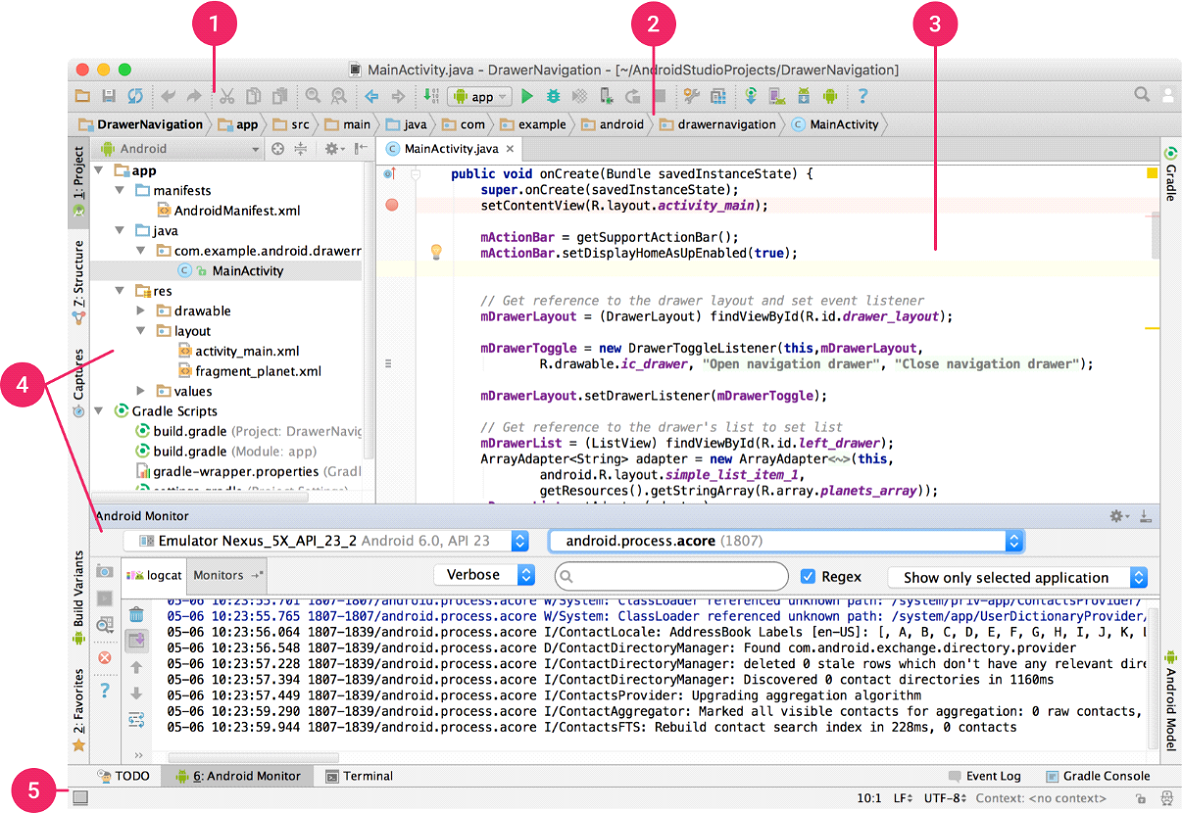
\includegraphics[scale=0.5]{slike/AndroidStudio.png}

\newpage

\section{Rešitev}
Aplikacija, ki sva jo naredila je sestavljena iz treh oken.
Prvo okno je vstopno okno v aplikacijo in ponuja tri možnosti: pridobitev lokacije uporabnika, prikaz vstopnih točk glede na katere se izračuna lokacija uporabnika in prikaz vseh vstopnih točk, ki jih aplikacij najde.
Za iskanje vstopnih točk se uporablja Wireless service za iskanje lokacije uporabika pa Location service.

Ob kliku na opcijo "dostopne točke" pridobimo RSSI vrednosti dostopnih točk, katerih lokacija je znana. Za tem se vrnemo na začetni zaslon in kliknemo na opcijo "Kje se nahajam?" ta opcija nam iz prej izmerjenih RSSI vrednosti in znanih lokacij dostopnih točk v prostoru izračuna pozicijo, kjer se nahajamo, prav tako pa nam poda še nekaj drugih podatkov, kot so: BSSID dostopne točke, njena lokacija ter izračunana razdalja do te dostopne točke.

\subsection{Izračun oddaljenosti Dostopne Točke}
Največjo težavo sva imela z določanjem razdalje do dostopne točke glede na RSSI vrednost. Našla sva več možnih načinov izračuna.

Prvi, ki sva ga poskusila implementirati je bil izpeljan iz Free-space path loss formule \cite{freespace}. Pri tej formuli sva opazila, da so vrednosti v bližini dostopne točke v primeru da ni veliko ovir, kar pomeni do nekje ene stene med dostopno točko in sprejemnikom so bili izračuni kar precej točni. Pri izračunu razdalje do dostopnih točk do katerih je bilo veliko ovir in zato tudi RSSI zelo nizek(v območju -70 in manj) pa je razdalja narasla na zelo veliko. 
Zaradi tega problema sva se odločila, do poskusiva poiskati drugo rešitev.
Tu naj omenim da, nisva mogla biti veliko na Fakulteti in tako imeti dostopa do bolj odprtega prostora z veliko dostopnimi točkami, kjer bi mogoče ta algoritem deloval bolje oz. bil dober za uporabo.

Naslednji, ki sva ga implementirala je bil način, za preračunavanje razdalje glede na procentno moč izmerjenega signala ter maximalni doseg dostopne točke \cite{trilateriationTechnique}. Izmerila sva maksimalen doseg izven vseh treh dostopnih točk skozi največ preprek, kar nama je dalo maximalen doseg nekje 15 metrov. vendar ta formula ni bila vredu, saj se signal z oddaljenostjo ne zmanjšuje linearno. Poskusila sva nekaj logaritmičnih funkcij in ugotovila, da sva najbolj točen rezultat dobila z logaritmom osnove 10 dobljenega signala.

\begin{figure}[htb]
\centering
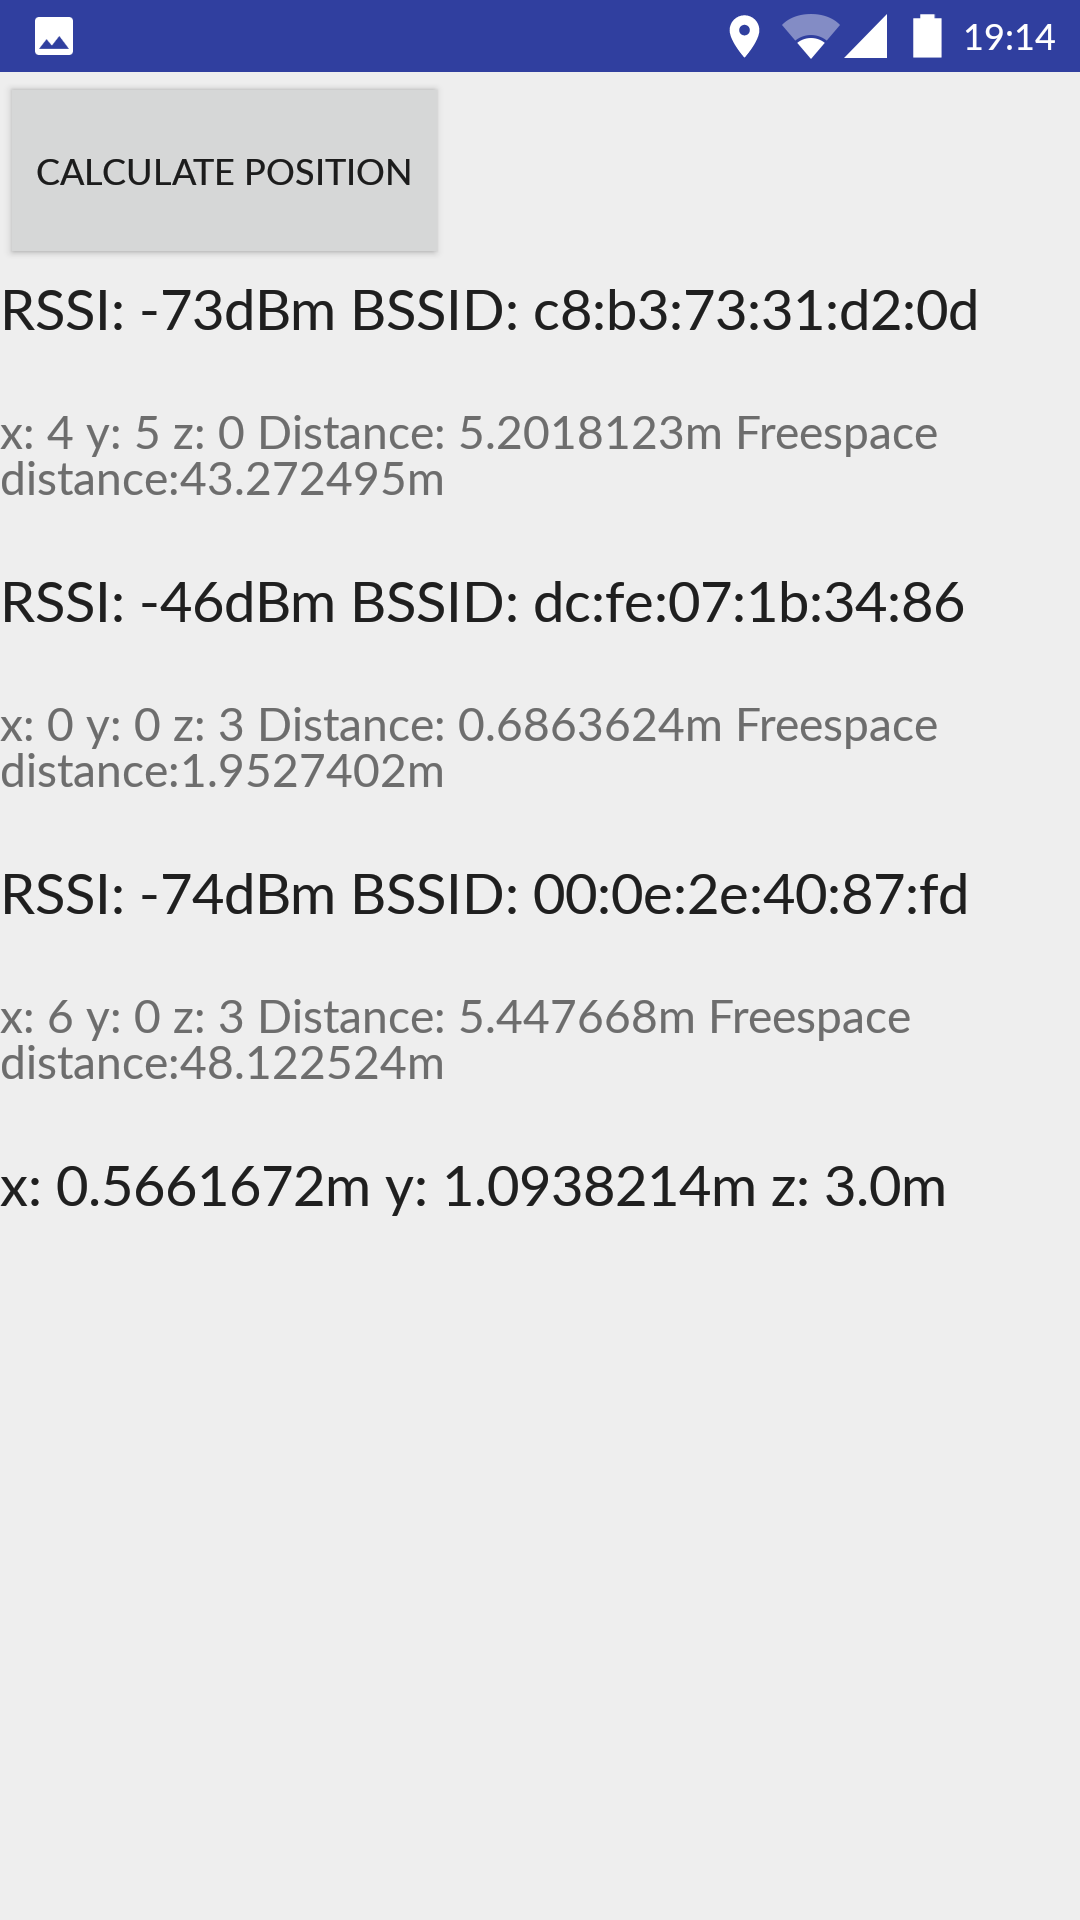
\includegraphics[scale=0.15]{slike/freespace1.png}
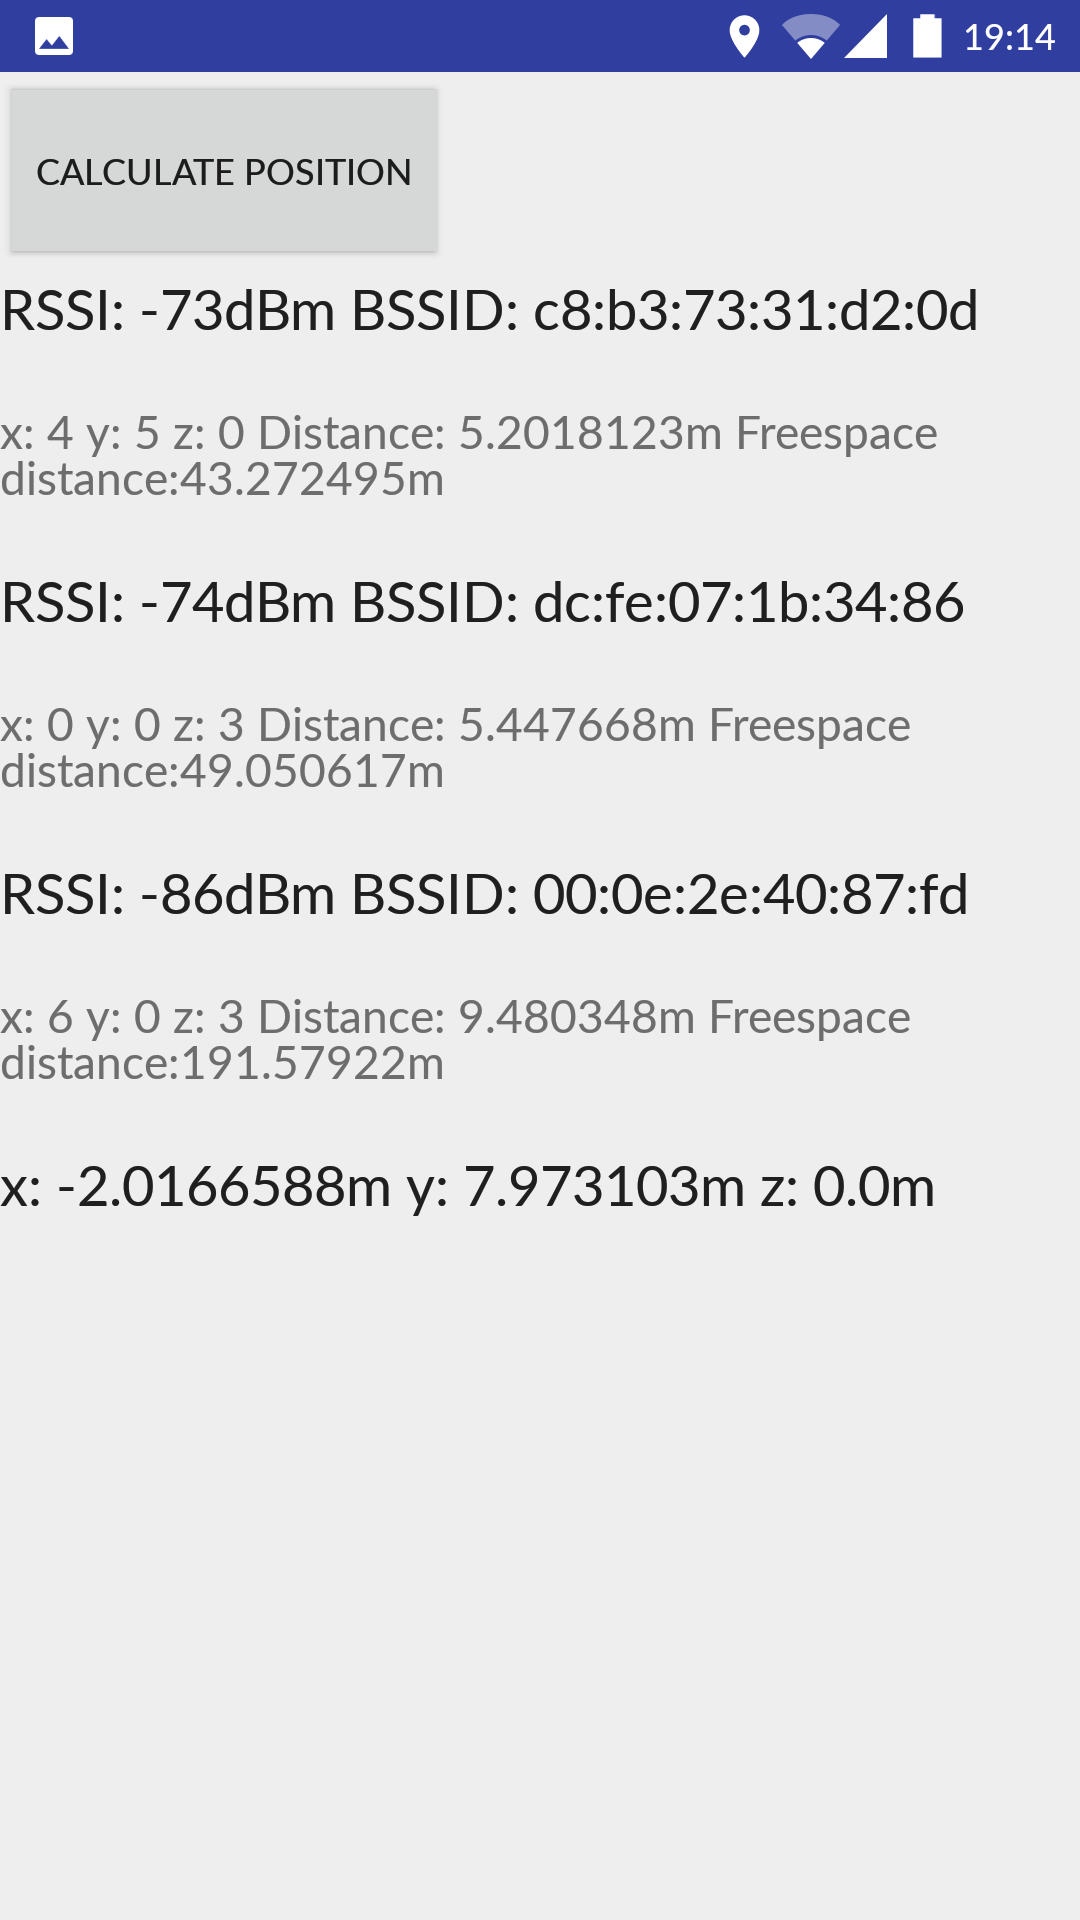
\includegraphics[scale=0.15]{slike/freespace2.png}
\caption{Iz zgornjih slik je razvidna napaka pri računanju razdalje z Free-space path loss algoritmom, ki je na sliki označen kot "Freespace distance" v primerjavi z končnim izbranim algoritmom katerega rezultat je označen kot "Distance". Vidimo tudi, da je na levi sliki pri majhni RSSI vrednosti algoritem kar točen, pri večjih pa hitro zbeži v velike vrednosti.}
\end{figure}


\subsection{Izračun lokacije}
Izračun lokacije sva uporabila Trilateracijo \cite{trilateration}.
Podroben opis rešitve. Sem spadajo načrtovanje, struktura omrežja, opis sprogramiranih modulov, konfiguracije usmerjevalnikov in omrežij.

\begin{figure}[htb]
\centering
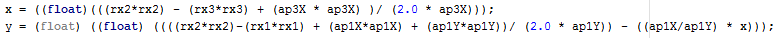
\includegraphics[scale=0.8]{slike/trilinerationCalculation.png}
\caption{Iz}
\end{figure}

\section{Rezultati}
Podroben opis rezultatov in pregled grafov performančne analize.

\section{Zaključek}
Z najino aplikacijo je bil dosežen željen cilj, ki sva si ga postavila. Spoznala sva, da je točen algoritem zelo težko narediti, najbolj to dokazuje izguba oz spreminjanje RSSI vrednosti zaradi preprek med odajnikom in sprejemnikom ter odbijanja signala. V primeru odprtih prostorov brez veliko preprek so algotirmi veliko bolj dovršeni in točni,v primeru kot sva ga imela midva pa je problem veliko bolj težaven, saj prihaja do veliko večjih napak že pri merjenju RSSI vrednosti.
Ali ste izpolnili cilje in možne nadaljne nadgradnje. Pri samem opisu rešitve se običajno sklicujemo na reference, npr.

\pagebreak
\bibliographystyle{plain}
\bibliography{references}

\end{document}











